\documentclass[tikz,border=3pt]{standalone}
\usepackage[T1]{fontenc}
\usepackage{mathptmx}
\usepackage{tikz,pgfplots}
\usetikzlibrary{arrows.meta,positioning,calc,fit,backgrounds,shapes.geometric}
\pgfplotsset{compat=1.18}
\definecolor{forest}{HTML}{346E57}
\definecolor{sage}{HTML}{E8EFEA}
\definecolor{clay}{HTML}{AC653F}
\definecolor{sand}{HTML}{F4EAE2}
\definecolor{ink}{HTML}{252525}
\definecolor{light}{HTML}{F5F5F3}
\definecolor{gridgray}{HTML}{D8DAD6}
\tikzset{box/.style={draw=ink!70,line width=.5pt,rectangle,rounded corners=1pt,fill=white,align=center,font=\fontsize{11}{12}\selectfont,inner sep=6pt}, flow/.style={-{Latex[length=2.4mm]},line width=.7pt,draw=ink!80}, data/.style={flow,densely dashed,draw=forest}, label/.style={font=\fontsize{10}{11}\selectfont,fill=white,inner sep=2pt,align=center}}
\hyphenpenalty=10000\exhyphenpenalty=10000\begin{document}
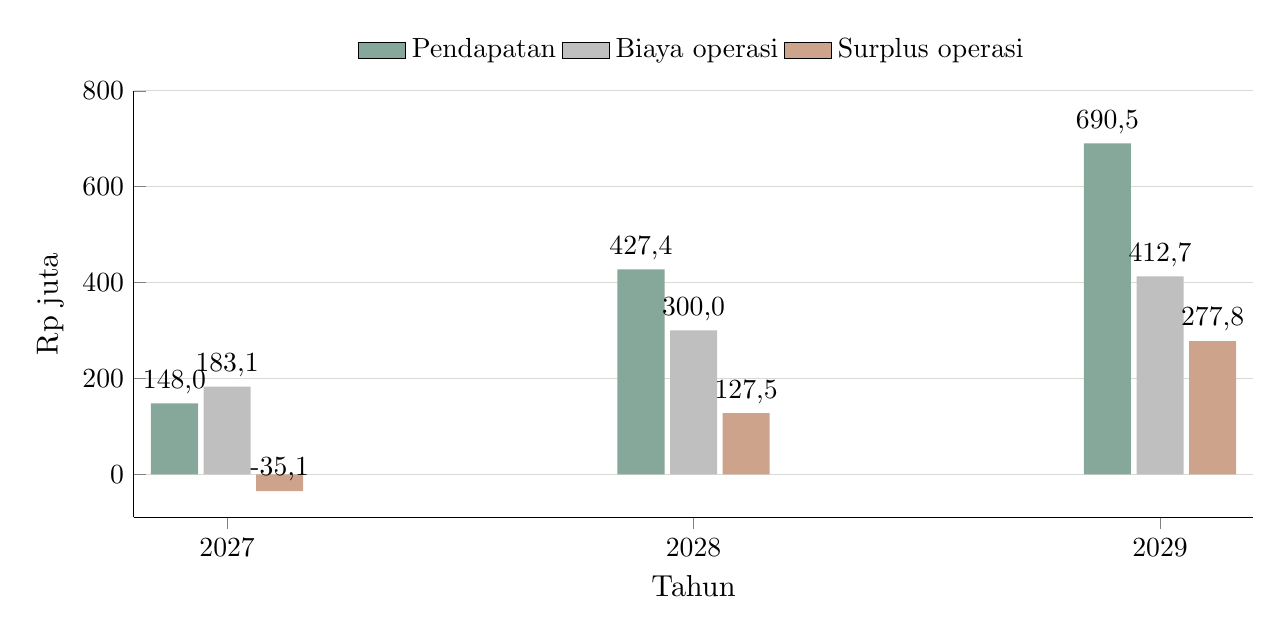
\begin{tikzpicture}\begin{axis}[width=15.8cm,height=7cm,ybar,bar width=17pt,ymin=-90,ymax=800,xtick={2027,2028,2029},xticklabels={2027,2028,2029},xlabel={Tahun},ylabel={Rp juta},axis lines*=left,ymajorgrids=true,grid style={gridgray},legend style={draw=none,at={(.5,1.04)},anchor=south,legend columns=3,font=\fontsize{10}{11}\selectfont},tick label style={font=\fontsize{10}{11}\selectfont},label style={font=\fontsize{11}{12}\selectfont},nodes near coords,nodes near coords style={font=\fontsize{10}{11}\selectfont,text=black},point meta=explicit symbolic]
\addplot[fill=forest!60,draw=none,area legend]coordinates{(2027,147.9600)[148,0](2028,427.4400)[427,4](2029,690.4800)[690,5]};\addlegendentry{Pendapatan}
\addplot[fill=black!25,draw=none,area legend]coordinates{(2027,183.0980)[183,1](2028,299.9720)[300,0](2029,412.7240)[412,7]};\addlegendentry{Biaya operasi}
\addplot[fill=clay!60,draw=none,area legend]coordinates{(2027,-35.1380)[-35,1](2028,127.4680)[127,5](2029,277.7560)[277,8]};\addlegendentry{Surplus operasi}
\end{axis}\end{tikzpicture}
\end{document}
